\documentclass[reprint,amsmath,amssymb,aps]{revtex4-2}

\usepackage{graphicx}
\usepackage{amsmath,amssymb,amsfonts}
\usepackage{dcolumn}
\usepackage{bm}
\usepackage{siunitx}
\sisetup{separate-uncertainty=true}
\usepackage[colorlinks,allcolors=blue]{hyperref}
\usepackage{cleveref}
\crefname{equation}{}{}
\crefname{figure}{Fig.}{Figs.}
\crefname{table}{Table}{Tables}
\usepackage{svg}





\begin{document}
\title{Testing Newton's second law with cart and mass}
\author{Sharone Krasnopolsky}
\email{Contact author: 426skrasnopolsky@frhsd.com}
\author{Timur Neyir}
\author{Brady Gorelczenko}
\affiliation{Science \& Engineering Magnet Program, \href{https://manalapan.frhsd.com/}{Manalapan High School}, Englishtown, NJ 07726 USA}
\date{\today}

\begin{abstract}
Newton’s second law states that force equals mass times acceleration ($F=ma$)
In our experiment, we used varying masses attached to a cart and pulley system in order to
examine the relationship between mass, acceleration, and force. We found that the relationship
between force and acceleration is proportional, supporting Newton’s second law.
\end{abstract}

\keywords{keywords here}

\maketitle

\section{Introduction}
Newton’s second law of motion states that acceleration of an object is directly proportional to the net force acting on that object and is inversely proportional to its mass:
\begin{equation}
F = ma,
\end{equation}
where $F$ is the net force, $m$ is the mass, and $a$ is the acceleration. In this experiment, we investigate the relationship between force, mass, and acceleration by analyzing the motion of a cart while it is being pulled over a pulley by a hanging mass. By varying the mass of the hanging mass, we examine how the change in force impacts the cart’s acceleration. We hypothesize that if the mass of the hanging weight is increased, then the acceleration of the cart will increase proportionally, in accordance with Newton's second law of motion, which states that acceleration is directly proportional to the net force applied and inversely proportional to the mass of the object.






\section{Methods and Materials}
The experiment used a \qty{0.500}{\kilo\gram} PASCO collision cart and a \qty{1.2}{\meter} long PASCO aluminum dynamics track. We used a \qty{0.200}{\kilo\gram} weight, a \qty{0.500}{\kilo\gram} weight, a \qty{1.000}{\kilo\gram} weight, a \qty{1.200}{\kilo\gram} weight, and a \qty{1.500}{\kilo\gram} weight as our hanging weights. In addition, we also used a PASCO ``super 
pulley with mounting rod'' as a pulley and a string to connect the weight to the cart. Our procedure started with setting up the track with the cart on top and the pulley hanging off the side as shown in \cref{fig:1} and \cref{fig:2}.

\begin{figure}
\caption{Track used in experiment}
\label{fig:1}
\end{figure}

\begin{figure}
\caption{Pulley where string is pulled, on the left is the cart, on the right, masses are hung}
\label{fig:2}
\end{figure}
  
\begin{figure}
\begin{center}
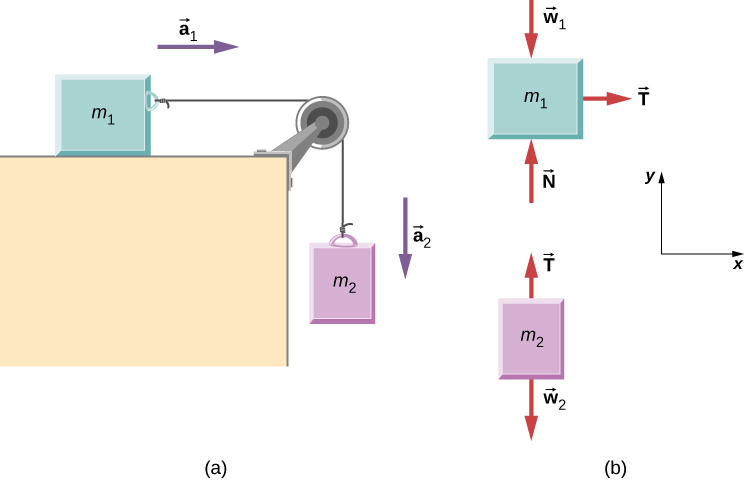
\includegraphics[width=\columnwidth]{CNX_UPhysics_06_01_Table.jpg}
\end{center}
\caption{Free-Body Diagram of the system in motion utilizing an ideal pulley, from \url{https://pressbooks.online.ucf.edu/phy2048tjb/chapter/6-1-solving-problems-with-newtons-laws/}}
\label{fig:3}
\end{figure}

We attached the \qty{0.200}{\kilo\gram} weight to the cart and pulled the cart back \qty{0.45}{\meter} from the pulley. The cart was then released and was allowed to freely accelerate until it reached the end of the track. In total, we took three trials for each of the five weights (\qtylist{0.200;0.500;1.000;1.200;1.500}{\kilo\gram}) for a total of 15 trials. During the trials, we measured the amount of time it took for the cart to travel \qty{0.45}{\meter} and recorded the data. Using the data, we calculated the tension force exerted on the cart using the formula $F=ma$. To calculate the acceleration, we used the equation $a=2d/t^2$ to find the acceleration.

\begin{figure}
\begin{center}
\includesvg[width=\columnwidth]{fig4.svg}
\end{center}
\caption{Graph that shows the mass of the weight ($x$) and time it took for the cart to reach the end of the track ($y$)}
\label{fig:4}
\end{figure}





\section{Results}
By taking the average times for each mass, we perform the equation $d = \frac{1}{2} a t^2$, which can be rearranged into, $a=2d/t^2$ to calculate the acceleration of the cart.
% latex table generated in R 4.4.2 by xtable 1.8-4 package
% Sat Nov 30 17:19:46 2024
\begin{table}
\begin{center}
\begin{ruledtabular}
\begin{tabular}{ccc}
$m_2$, \unit{\kilo\gram} & $t$, \unit{\second} & $a$, \unit{\meter\per\second\squared} \\ 
\colrule
\num{0.200} & \num{0.56\pm0.02} & \num{2.84\pm0.15} \\ 
\num{0.500} & \num{0.46\pm0.02} & \num{4.27\pm0.37} \\ 
\num{1.000} & \num{0.36\pm0.01} & \num{6.82\pm0.21} \\ 
\num{1.200} & \num{0.31\pm0.01} & \num{9.17\pm0.33} \\ 
\num{1.500} & \num{0.30\pm0.01} & \num{10.0\pm0.7} \\ 
\end{tabular}
\end{ruledtabular}
\end{center}
\end{table}


%FTheoretical = 0.5kg X 9.8 m/s2 = 4.9N
%F200g = 0.5kg X 2.836 m/s2 = 1.418N
%F500g = 0.5kg X 4.253 m/s2 = 2.127N
%F1000g = 0.5kg X 6.819 m/s2 = 3.409N
%F1200g= 0.5kg X 9.169m/s2 = 4.585
%F1500g= 0.5kg X 10 m/s2 = 5 N






\section{Discussion}
In this experiment, we investigated Newton’s second law, $F=ma$, by examining how varying weights influenced the acceleration of a cart. Our data demonstrates a strong proportional relationship between force and acceleration, with calculated values aligning closely with theoretical predictions.

The slight discrepancies between theoretical and experimental force values can be attributed to friction on the track, which likely reduced the net force acting on the cart. Additionally, timing inaccuracies over short distances may have introduced minor errors in measuring the acceleration. Pulley inefficiencies, such as resistance or string tension losses, could also have contributed to the observed deviations.

These findings validate Newton’s second law while highlighting areas for improvement in the experimental setup. Implementing a frictionless track, using a more precise timing mechanism, and optimizing the pulley system could help achieve results that more closely match theoretical values.




\section{Acknowledgements}
We thank several anonymous reviewers for their helpful comments on our manuscript. 

SK set up the track, measured the time it took for the cart to travel \qty{0.45}{\meter}, and wrote the abstract, introduction, methods and materials, and acknowledgements. TN also helped set up the track, recorded the results, did all calculations, and wrote results and discussions. BG helped prepare experiment materials and helped with pre-trial measurements. 




% References
%[1] P. Tipler, G. Mosca, Physics for Scientists and Engineers, Extended (W.H. Freeman and Company, United States, 2004)
%Free Body Diagram of the experimental setup found here: 
%https://pressbooks.online.ucf.edu/phy2048tjb/chapter/6-1-solving-problems-with-newtons-laws/

%\bibliographystyle{abbrvnat}
\bibliography{lab.bib}
\end{document}